\documentclass{article}[12 pt]
\usepackage{amssymb}
\usepackage{amsthm}
\usepackage{amsmath}
\usepackage{appendix}
\usepackage{array}
\usepackage{geometry}
\usepackage{enumitem}
\usepackage{graphicx}
\usepackage{subfig}
\usepackage{caption}
\usepackage{url}
\usepackage{float}
\usepackage{pdfpages}
\usepackage{shortvrb}
\usepackage{mathtools}
\usepackage{multirow}
\usepackage{hyperref}
\usepackage{commath}
\usepackage{tabularx}


\def\BibTeX{{\rm B\kern-.05em{\sc i\kern-.025em b}\kern-.08em
		T\kern-.1667em\lower.7ex\hbox{E}\kern-.125emX}}

\graphicspath{{"K:/University of Florida/Classes/2019_08_Principe_Deep_Learning/Homework/HW01/Report/Images/"}{"C:/Users/Conma/Desktop/HW01/Report/Images/"}{"/media/cmccurley/0000-0001/University of Florida/Classes/2019_08_Principe_Deep_Learning/Homework/HW01/Report/Images/"}}
\geometry{margin=1 in}

\newcommand{\smallvskip}{\vspace{5 pt}}
\newcommand{\medvskip}{\vspace{30 pt}}
\newcommand{\bigvskip}{\vspace{100 pt}}
\newcommand{\tR}{\mathtt{R}}




\begin{document}
	
\begin{center}
	\textbf{\Large Connor McCurley} \\
	EEE 6814 \qquad \textbf{\large Homework 1} \qquad Fall 2019 
\end{center}




\section*{Question 1}
Question 1 asked us to hand-design a ANN architecture which is capable of creating discrimination regions resembling the mask shown in the handout.  Based on the design, it was determined that the discriminator could be created from a two-hidden-layer network shown in Figure \ref{fig:architectureQ1}.  

\begin{center}
	\begin{figure}[h]
		\centering
		\includegraphics[width=0.75\textwidth]{"Architecture_Q1"}
		\caption{Architecture implemented to solve the mask problem.  The network implements a two hidden layer MLP with two input units, 13 units in the first hidden layer, 4 hidden units in the second layer, and 1 output neuron. Sign functions were used for activations in the network. }
		\label{fig:architectureQ1}
	\end{figure}
\end{center}
\noindent
This architecture defines a two hidden layer MLP with two input features, 13 hidden units in the first layer (3 for the nose, 4 for the mouth, 2 for each eye, and two shared between the eyes), 4 hidden units in the second hidden layer (to determine if a sample is contained in one of the desired discrimination regions), and a single neuron in the output.  To select the parameters of the network by hand, I used the following arbitrary weight relationship defined in class:

\begin{align*}
	x_2 = -\frac{w_1}{w_2}x_1 - \frac{b}{w_2}
\end{align*}

\noindent
where $x_1$ and $x_2$ are inputs, $w_1$ and $w_2$ are corresponding weights, and $b$ is a bias term.  From this, I determined the weights for the units in the first hidden layer as:

\begin{table}[H]
	\caption{Weights in the First Hidden Layer}
	\label{tab:WeightsFirstHiddenLayer}
	\begin{center}
		\begin{tabularx}{\textwidth}{ |X|X|X|X| } 
			\hline
			\textbf{Mask Region} & \textbf{$w_1$} & \textbf{$w_2$} & \textbf{Bias}\\
			\hline
			Nose & 0 &  1& 1\\
			\hline
			  & 1 &  1 & 0\\
			\hline
			  & -1 &  1 & 0\\
			\hline
			Mouth & 0 & 1 & 3\\
			\hline
			 & 0 &  1& 4\\
			\hline
			 & 1 &  0 & 3\\
			 \hline
			 & 1 &  0 & -3\\
			 \hline
			 Left Eye & 1 & 0 & 5\\
			 \hline
			 & 1 &  0 & 4\\
			 \hline
			 Right Eye & 1 & -5 & 3\\
			 \hline
			 & 1 &  0 & -4\\
			 \hline
			 Both Eyes & 0 & 1 & -5\\
			 \hline
			 & 0 &  1 & -4\\
			 \hline
		\end{tabularx}
	\end{center}
\end{table}

\noindent To test the correctness of my parameters, I defined a test dataset and passed it through the network.  The outputs of each neuron in the second hidden layer are shown in Figure \ref{fig:maskComponents}, where yellow represents a value of 1, and blue a value of -1.



\begin{figure}[H]%
	\centering
	\subfloat[Nose]{{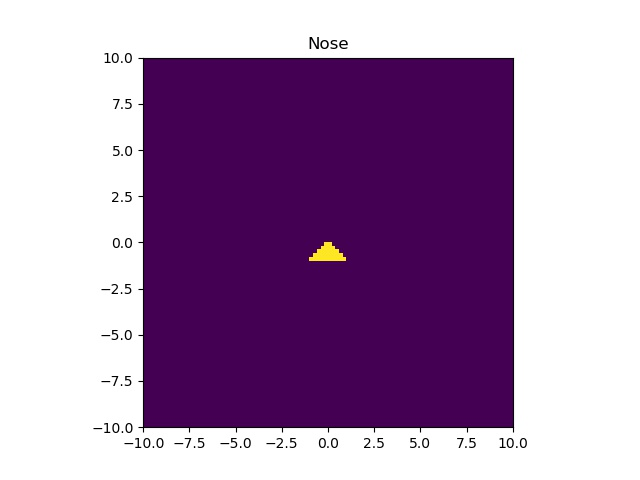
\includegraphics[width=5cm]{Nose} }}%
	\qquad
	\subfloat[Mouth]{{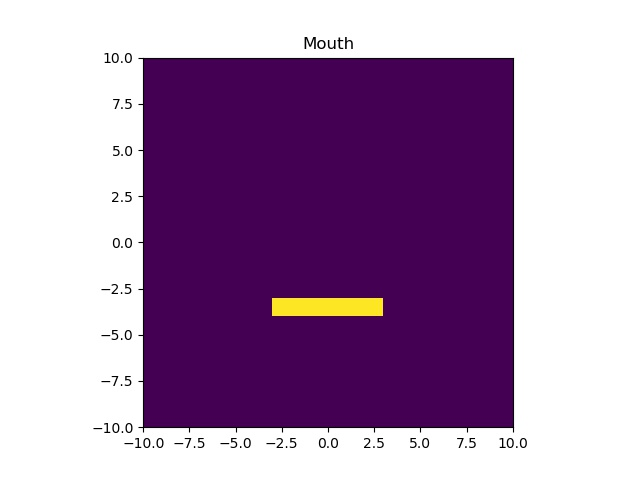
\includegraphics[width=5cm]{Mouth} }}%
	\qquad
	\subfloat[Left Eye]{{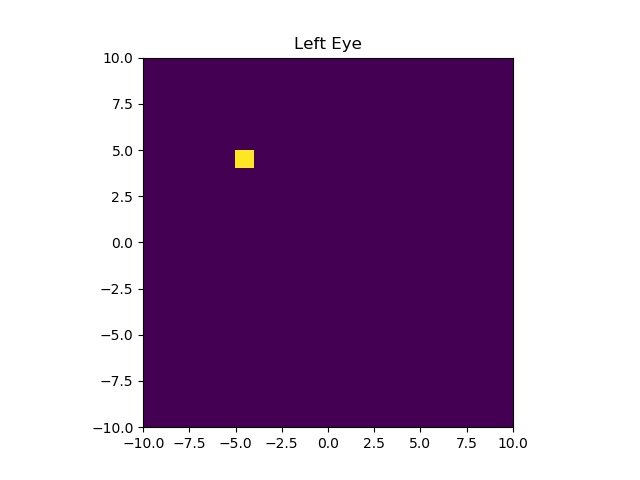
\includegraphics[width=5cm]{LeftEye} }}%
	\qquad
	\subfloat[Right Eye]{{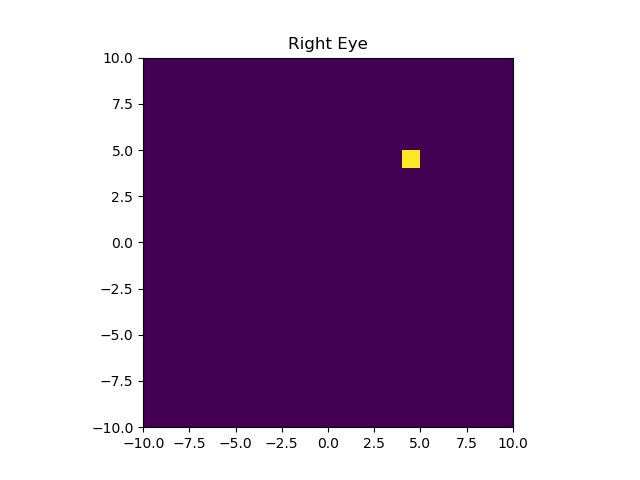
\includegraphics[width=5cm]{RightEye} }}%
	\caption{Outputs of the second hidden layer in the ``mask network''.  It can be observed that each unit in this layer determines whether a sample falls within a desired mask region.}%
	\label{fig:maskComponents}%
\end{figure}

\noindent
From there, I hand-selected a few points both within and outside of each desired region, passed them through the network, and hand-plotted them in the ``new parameter space".  The process was then repeated as above and the weights in the second hidden layer were found to be:

\begin{table}[H]
	\caption{Weights in the Second Hidden Layer}
	\label{tab:WeightsSecondHiddenLayer}
	\begin{center}
		\begin{tabularx}{\textwidth}{ |X|X|X|X|X|X| } 
			\hline
			\textbf{Mask Region} & \textbf{$w_1$} & \textbf{$w_2$} & \textbf{$w_3$} & \textbf{$w_4$} & \textbf{Bias}\\
			\hline
			Nose & 2 &  -0.5 & -0.5 & 0 & -2\\
			\hline
			Mouth & -3 & 3 & 0.5 & -1 & -7\\
			\hline
			Left Eye & -3 & 3 & 0.5 & -1 & 7\\
			\hline
			Right Eye & -3 & 3 & -2 & 2 & -6\\
			\hline
		\end{tabularx}
	\end{center}
\end{table}

\noindent
When provided the same test set, this MLP architecture was able to generate the desired ``mask" discrimination regions.\\

\noindent
Question 1 also posed the question as to whether the same goal could be achieved with a single hidden layer network.  I would answer that it could be done if the output layer was truncated and the outputs of the neurons currently in the second hidden layer were be used to create an output vector.  An extra neuron, however, would need to be added in the output layer as a ``background'' discriminator. 


\section*{Question 2}

For question 2, I designed a single hidden layer MLP to solve the Star Problem (Figure \ref{fig:Q2Data}), and coded backpropagation (code included) to train the network.  For this architecture, I chose a single hidden layer MLP with two inputs, 4 hidden units, and a single output neuron, as shown in Figure \ref{fig:architectureQ2}.  

\begin{center}
	\begin{figure}[H]
		\centering
		\includegraphics[width=0.4\textwidth]{"Q2_data"}
		\caption{Training data points for the Star Problem.  Class labels are denoted by color. }
		\label{fig:Q2Data}
	\end{figure}
\end{center}

\begin{center}
	\begin{figure}[H]
		\centering
		\includegraphics[width=0.4\textwidth]{"Architecture_Q2"}
		\caption{Architecture implemented to solve the Star Problem.  The network consists of a single hidden layer MLP with two input units, 13 units in the first hidden layer, 4 hidden units in the second layer, and 1 output neuron. Sigmoid activation functions were used at each neuron in the network. }
		\label{fig:architectureQ2}
	\end{figure}
\end{center}

\noindent
After my first round of training, I obtained the following results:
\begin{center}
	\begin{figure}[H]
		\centering
		\includegraphics[width=0.75\textwidth]{"Q2_decision_regions_inexact"}
		\caption{Decision regions learned by the single hidden layer network shown in Figure \ref{fig:architectureQ2}.  The regions partially solve the Star Problem, but fail for out-of-sample data points. }
		\label{fig:Q2RegionsInexact}
	\end{figure}
\end{center}

\begin{center}
	\begin{figure}[H]
		\centering
		\includegraphics[width=0.5\textwidth]{"Q2_learning_curve_inexact"}
		\caption{Learning curve for the network shown in Figure \ref{fig:architectureQ2}.  This shows that the network's training error falls below 0.002 after approximately 1000 iterations of training with a learning rate of 0.8.}
		\label{fig:Q2RegionsInexact}
	\end{figure}
\end{center}

\begin{center}
	\begin{figure}[H]
		\centering
		\includegraphics[width=0.5\textwidth]{"Q2_weight_tracks_inexact"}
		\caption{Weight tracks for the network shown in Figure \ref{fig:architectureQ2}.  This shows that the network's weights converge after approximately 1000 iterations of training.}
		\label{fig:Q2RegionsInexact}
	\end{figure}
\end{center}



\noindent
Both the weight tracks (which stabilized) and the MSE learning curve demonstrated that the network obtained good performance on the training data.  However, when provided out-of-sample data, the model did not generalize to the desired discrimination regions.  It occurred to me that, to allow the model to more-easily discover our desired discrimination regions, we could force some of the weights to 0 so that the network would learn only vertical and horizontal lines.  After enforcing these constraints, the network learned the following:

\begin{center}
	\begin{figure}[H]
		\centering
		\includegraphics[width=0.75\textwidth]{"Q2_decision_regions_exact"}
		\caption{Decision regions learned by the single hidden layer network shown in Figure \ref{fig:architectureQ2}, with constraints to learn only horizontal and vertical decision boundaries.  The regions perfectly solve the Star Problem. }
		\label{fig:Q2RegionsInexact}
	\end{figure}
\end{center}

\begin{center}
	\begin{figure}[H]
		\centering
		\includegraphics[width=0.5\textwidth]{"Q2_learning_curve_exact"}
		\caption{Learning curve for the network shown in Figure \ref{fig:architectureQ2} with constraints to learn only horizontal and vertical decision boundaries.  This shows that the network's training error falls below 0.002 after approximately 1200 iterations of training with a learning rate of 1.2.}
		\label{fig:Q2RegionsInexact}
	\end{figure}
\end{center}

\begin{center}
	\begin{figure}[H]
		\centering
		\includegraphics[width=0.5\textwidth]{"Q2_weight_tracks_exact"}
		\caption{Weight tracks for the network shown in Figure \ref{fig:architectureQ2} with constraints to learn only horizontal and vertical decision boundaries.  This shows that the network's weights converge after approximately 1200 iterations of training.}
		\label{fig:Q2RegionsInexact}
	\end{figure}
\end{center}

\noindent
These results shows that the network was able to perfectly learn the star problem.  As a side note, corners of the discrimination region look a bit rounded due to the number of samples in the test grid.   

\begin{thebibliography}{00}
	\bibitem{Principe}Principe, Jose C., Euliano, Niel R., Lefebvre, W. Curt. "Chapter III- Multilayer Perceptrons," in Neural and Adaptive Systems: Fundamentals Through Simulation, 1997
\end{thebibliography}

\end{document}
